\documentclass[conference, compsocconf]{IEEEtran}
%\documentclass{llncs}

\newif\ifnoTBD \noTBDfalse

% Uncomment to remove TBD macros
%\noTBDtrue

\ifnoTBD
\def\TBD#1{\typeout{TBD not done: #1}}
\else
\def\TBD#1{\textcolor{blue}{TBD: #1}}
\AtEndDocument{\typeout{ *** ATTENTION: compilation is in DRAFT
    mode. There might still be TBD that appear in the document ***}}
\fi

\usepackage[usenames]{color}
\usepackage{xspace}
\usepackage{listings}
%\usepackage{type1cm}
\usepackage{eso-pic}
\usepackage{subfigure}
\usepackage{multirow}
\usepackage{url}
\usepackage{latexsym}
%\usepackage{hyperref}
\usepackage{comment}
\usepackage{graphicx}
\usepackage{algorithmic}
\usepackage{algorithm}
%\usepackage{amsthm}
%\usepackage{amsfonts} 
%\usepackage{amssymb}
%\usepackage{amsmath} 
\usepackage{underscore}
\usepackage{color}
\usepackage[table]{xcolor}
\usepackage{flushend}
\usepackage{setspace}

%\setlength{\oddsidemargin}{0in}   % origin is (1",1") from top-left corner
%\setlength{\evensidemargin}{0.0in}
%\setlength{\textwidth}{6.5in}
%\setlength{\textheight}{9in}
%\setlength{\topmargin}{0.0in}
%\setlength{\headheight}{0pt}
%\setlength{\headsep}{0pt}

\newcommand{\ompi}{Open\,MPI\xspace}
\newcommand{\ftla}{FT-LA\xspace}
\newcommand{\scalapack}{ScaLAPACK\xspace}
\newcommand{\abft}{ABFT\xspace}
\newcommand{\cof}{CoF\xspace}
\newcommand{\ulfm}{ULFM\xspace}
\newcommand{\mpifunc}[1]{{\tt #1}}

%\doublespacing

\begin{document}

\title{Toward Recovery Capabilities in Message Passing Environments}
\author{
  \IEEEauthorblockN{Wesley Bland}
  \IEEEauthorblockA{Department of Electrical Engineering and Computer Science\\
  					University of Tennessee, Knoxville\\
					wbland@icl.utk.edu}
}
%\author{Wesley Bland}
%\institute{Department of Electrical Engineering and Computer Science\\
%University of Tennessee, Knoxville\\
%wbland@icl.utk.edu}

\maketitle

\section{Dissertation Statement}\label{sect:dissertation}

The goal of the dissertation is to demonstrate novel methods of fault tolerance
supporting Algorithm Based Fault Tolerance (ABFT) for large scale systems using
the message passing paradigm with extensions to facilitate concurrent approaches
to cope with failures. By allowing applications to continue execution after a
hardware failure, algorithms can support larger scale and longer running
executions previously found to be unattainable.

\section{Motivation}
\label{sect:motivation}

A major concept followed in the design of any type of parallel programming paradigm, and
this in order to provide a meaningful and understandable programming approach,
is the avoidance of any potential deadlocks. In addition to this critical
requirement the mechanisms involved in the fault management were build with the
goal of flexibility, simplicity and performance.

Clearly the most important point, no MPI call (point-to-point or collective) can
block indefinitely after a failure, but must either succeed or raise an MPI
error. Fault tolerance at the application level is impossible if the application
cannot regain full control of the execution after a process failure. The MPI
library must guarantee that it will automatically stabilize itself following a
process failure, and provide the tools necessary for the application to resolve
its own deadlock scenarios on an application specific basis.
% The \ulfm proposal implements this idea with the \mpifunc{MPI\_COMM\_REVOKE}
% construct, detailed in Section~\ref{sect:newmpi}.

Second, the API should allow varied fault tolerant models to be built. MPI has
been conceived with the goal of portability and extendability, and have been
constructed to support libraries leveraging existing MPI constructs to create
more abstractions or tighter integration with libraries. Maintaining this design
strength was paramount for \ulfm, and it provides this capability so other
levels of consistency can be supported as needed by higher-level
concepts. Transactional fault tolerance, strongly uniform collective operations,
and other FT techniques can all therefore be built upon the proposed set of
constructs.

An API should be easy to understand and use in common scenarios, as complex
tools have a steep learning courve and a slow adoption by the targeted
communities. To this end, the number of newly proposed constructs have been
reduced to five (along with nonblocking variants). These five functions provide
the minimal set of tools to implement fault tolerant applications and libraries.

Two major pitfalls must be avoided when implementing these concepts: jitter
prone, permanent monitoring of the health of peers a process is not actively
communicating with, and expensive consensus required for returning consistent
errors at all ranks.  The operative principle is that fault-related errors are
local knowledge, and are not indicative of the return status on remote
processes. Errors are raised at a particular rank, when based on local knowledge
it is known that a particular operation cannot complete because a participating
peer has failed.

\section{Related Work}\label{sect:related}

% Why coordinated checkpointing is no longer scalable

The current industry standard for failure handling is rollback recovery with
periodic checkpoints to disk, and many libraries have been implemented to
support this behavior~\cite{Duell:tr, Litzkow:1997wd, Plank:1994wz,
Zhong:2001tq}. This has been an effective recovery model for many years and
continues to be an area of research to prolong its
usefulness~\cite{BautistaGomez:2011hg, BuntinasFGCS2008, Elnozahy:2002p3769},
despite the increase in fault frequency and the hierarchization of the
underlying hardware architecture.  However as machines continue to scale,
concerns have been raised about the scalability of rollback
recovery~\cite{Cappello:2009hs}.  The time spent performing recovery operations
is expected to exceed the MTBF in the next generation of supercomputers, causing
any large-scale applications to enter a cycle of recovery where no useful
computation occurs.

% Resilience workshop report

In February 2012, the Department of Defense and Department of Energy conducted
research~\cite{Daly:2012vg} to outline the necessity for resilience at extreme
scale, specifically for exascale computing. They affirmed the likelihood that
exascale systems will have a shorter MTBF than existing systems. They also
recommended that ``a `light-weight' approach, i.e., effective and easy to
implement, is preferable to a `full-featured' alternative.'' By attempting fewer
features, each library can focus on creating a scalable and efficient
implementation while promoting simplicity and reducing unnecessary features. The
agencies also discussed possible redundancy approaches (discussed
in~\cite{BosilcaINRIARep7950, Ferreira:2011fb}), describing them as ``not
practical because they require 2-3x more energy''. The price of redundancy must
not only include the obvious loss of computing time from executing duplicate
codes across multiple processors, but also the up-front costs of purchasing
extra hardware on which to execute the redundancy.

% Describe ABFT

Out of these problems have arisen a new class of algorithms that allow different
methods of resilience. These algorithms support what is called Algorithm Based
Fault Tolerance (ABFT). They have been designed to support a recovery model that
does not require all processes to participate in the recovery simultaneously or,
perhaps, ever at all. Huang and Abraham first explored these
algorithms~\cite{Huang:1984kt} for soft errors in systolic arrays, but research
has expanded to create ABFT techniques for many algorithms~\cite{Du:2012je, Plank:1995hv}.

% RTS Proposal

To support these new algorithms, applications require support from their
libraries. One of the most popular communication libraries used by large scale
applications is the Message Passing Interface (MPI), the contents of which are
determined by the MPI Forum. The MPI Forum has previously considered proposals
to add fault tolerance capabilities to the MPI Standard. In 2011, a proposal was
brought forth~\cite{Hursey2011RTS} titled ``Run-Through Stabilization'' which
discussed a wide range of fault tolerance capabilities to provide for users by
defining the behavior of MPI following a process failure as well as introducing
new constructs to provide strong consensus between processes. The MPI Forum
decided to reject the proposal, but the work led to more research in the field
of resilience in MPI, including the work being proposed in
Section~\ref{sect:ulfm}.

% FT-MPI

Outside of the MPI Forum, work has been done to provide fault tolerance to MPI
applications. FT-MPI~\cite{FaggFTMPI} was an MPI-1 compliant implementation of
the MPI Standard which added new capabilities for fault tolerance. It included
automatic recovery models for failures including: shrinking MPI communicators to
automatically remove failed processes, leaving holes in the communicators while
allowing communication to continue, and destroying and rebuilding the
communicators to retain communication patterns and groups. FT-MPI was never
adopted into the MPI Standard but continued as a research project for many
years. 

\section{Checkpoint-on-Failure}\label{sect:cof}

% Teaser paragraph
Checkpoint-on-Failure (CoF)~\cite{Bland:2012tw} combines the familiarity of
checkpointing with the flexibility of \abft. As discussed in
Section~\ref{sect:related}, coordinated checkpointing is no longer considered a
scalable option for fault tolerance due to the increasing frequency and size of
the individual checkpoints. However, for some types of applications which can
take advantage of it, \cof can reduce the necessary number of checkpoints. In
the failure-free case, no checkpoints are made, and in all other cases, only the
optimal number of checkpoints are required.

% Define the "high-quality" implementation from the MPI Standard

The current MPI Standard (version 2.2~\cite{MPI22}) intentionally does not provide a
guideline for the behavior of the MPI library after a process failure. Section
2.8 states: ``\emph{MPI does not provide mechanisms for dealing with failures in
the communication system. [\ldots] Whenever possible, such failures will be
reflected as errors in the relevant communication call. Similarly, MPI itself
provides no mechanisms for handling processor failures.}'' Later, in the same
section: ``\emph{This document does not specify the state of a computation after
an erroneous MPI call has occurred. The desired behavior is that a relevant
error code be returned, and the effect of the error be localized to the greatest
possible extent.}'' Using these two sections from the standard, it is possible
to construct a minimal failure handling method using roll-forward recovery.

Section 8.3 (Error Handling) defines the behavior of a ``high quality''
implementation pertaining to error handling: ``\emph{A good quality
implementation will, to the greatest possible extent, circumscribe the impact of
an error, so that normal processing can continue after an error handler was
invoked.}'' By using a ``high quality'' MPI implementation as defined here, an
application will receive a notification from the MPI library through a custom
\mpifunc{MPI\_ERRHANDLER} when a failure occurs and before the library shuts
down operation. MPI makes no guarantee about the availability of the
communication library following a process failure, therefore standard
roll-forward recovery mechanisms are no longer possible. However, by using CoF
methods, an application still has an opportunity to save its state and exit
gracefully, then be restarted with the original number of processes and perform
recovery.

% Describe CoF in more detail

%\begin{algorithm*}
%\caption{The Checkpoint-on-Failure Protocol}
%\label{alg:on-demand-alg}\label{fig:cof-idea}
%\centering
%\begin{minipage}{.55\linewidth}
%	\begin{enumerate}
%		\item MPI returns an error on surviving processes 
%		\item Surviving processes checkpoint
%		\item Surviving processes exit
%		\item A new MPI application is started
%		\item Processes load from checkpoint (if any)
%		\item Processes enter \abft dataset recovery
%		\item Application resumes
%	\end{enumerate}
%\end{minipage}
%\hfill %\begin{minipage}{.39\linewidth}
%\includegraphics[width=\linewidth]{figures/cof-idea.pdf}
%\end{minipage}
%\end{algorithm*}

%Algorithm~\ref{alg:on-demand-alg}\footnote{Figure appeared
%in~\cite{Bland:2012tw}} presents the steps involved in the \cof method.
%Horizontal lines represent the execution of the MPI processes. 

The usage of the \cof model can be described as follows. When a failure
eliminates a process, other processes are notified and control is returned from
ongoing MPI calls. Surviving processes assume the MPI library is dysfunctional
as described in the MPI Standard and make no further calls to the MPI library
(in particular, they do not yet undergo \abft recovery). Instead, they
checkpoint their current state independently and abort. When all processes have
exited, the job is usually automatically terminated, and the user (or a managing
script, batch scheduler, runtime support system, etc.) can launch a new MPI
application, which reloads processes from checkpoint. In the new application,
the MPI library is functional and communication is once again possible; the
\abft recovery procedure is called to restore the data of the process(es) that
did not restart with a checkpoint (because they were the processes which
failed). When the global state has been repaired by the \abft procedure, the
application is ready to resume normal execution.

% Performance vs. periodic checkpointing

\cof has many advancements beyond traditional periodic checkpointing. First, it
is always optimized both in space and time. It takes checkpoints only after a
failure has occurred, meaning that there is no need to calculate an optimal
checkpoint interval~\cite{Daly:2006dy} or pause failure-free execution to write
state to disk. This can provide a measurable speedup in the application
performance, especially at scale because it reduces resource contention for the
I/O system. Also, because checkpoints are only written by processes which are
known to be alive, the checkpoint can be written to local stable storage rather
than requiring I/O be communicated between a remote, safe data store. The
overhead of \cof is also comparable to the standard overhead introduced by other
\abft techniques. The application might need to do extra computation, even in
the absence of failures, to maintain internal redundancy used to recover data
damaged by failures, however, this is necessary for all \abft techniques.

% MPI Requirements

\subsection{MPI Requirements for Checkpoint-on-Failure}\label{sec:interface}

\paragraph*{Regaining Control After Failures} In most MPI implementations,
\mpifunc{MPI\_ERRORS\_ABORT} is the default (and often, only functional) error
handler.  However, the MPI Standard also defines the error handler,
\mpifunc{MPI\_ERRORS\_RETURN} and provides mechanisms for custom error handlers
defined by the application. To support \cof, the MPI library should never
deadlock because of failures, but invoke the error handler, at least on
processes doing direct communications with the failed process. The error handler
takes care of cleaning up at the library level and returns control to the
application.

\paragraph*{Termination After Checkpoint} A process that detects a failure
ceases to use MPI. It checkpoints to storage, local or remote, and exits without
calling \mpifunc{MPI\_FINALIZE} (it may choose to call
\mpifunc{MPI\_COMM\_ABORT}, but this behavior is not required). Exiting without
calling \mpifunc{MPI\_FINALIZE} is an error from the MPI perspective, hence the
failure notification becomes fully propagated and MPI eventually calls the error
handler on all processes, which trigger their own checkpoint procedure and
termination.

\subsection{\ompi Implementation\label{sec:mpi}}

\ompi is an MPI 2.2 implementation architected such that it contains two main
levels, the runtime (ORTE) and the MPI library (OMPI). As with most MPI library
implementations, the default behavior of \ompi is to abort after a process
failure. This policy was implemented in the runtime system, preventing any kind
of decision from the MPI layer or the user level. The major change required by
the \cof protocol was to make the runtime system resilient, leaving the policy
for failure handling to the MPI library, and ultimately the user application.

\paragraph*{Resilient Runtime} The ORTE runtime layer provides an out-of-band
(OOB) communication mechanism that relays messages based on a routing policy.
Node failures not only impact the MPI communications, but also disrupt routing
at the OOB level. The default routing policy in ORTE has been amended to allow
for self-healing behaviors; this effort is not entirely necessary, but it avoids
the significant downtime imposed by a complete redeployment of the parallel job
with resubmission into execution queues. The underlying OOB topology is
automatically updated to route around failed processes. In some routing
topologies, such as a star, this is a trivial operation and only requires
excluding the failed process from the routing tables. For more elaborate
topologies, such as trees, the healing operation involves computing
the closest neighbors in the direction of the failed process and reconnecting
the topology through them. The repaired topology is not rebalanced, which could
result in improved performance but would disrupt expected communication
patterns, however it does retain complete functionality to allow the MPI
implementation to maintain internal communication and facilitate failure
notification. Although in-flight messages that were currently ``hopping''
through the failed processes are lost, other in-flight messages are safely
routed by the repaired topology. Thanks to self-healing topologies, the runtime
remains responsive, even when MPI processes leave.

\paragraph*{Failure Notification} The runtime has been further augmented with a
failure detection service. To track the status of the failures, an incarnation
number has been included in the process names. Following a failure, the name of
the failed process (including the incarnation number) is broadcasted over the
OOB topology. By including this incarnation number, we can identify transient
process failures, prevent duplicate detections, and track message status. ORTE
processes monitor the health of their neighbors in the OOB routing topology.
Process failure detection relies on a resilient broadcast operation that
overlays on the OOB topology. However, the underlying OOB routing algorithm has
a significant influence on failure detection and propagation time, as the
experiments will show. On each node, the ORTE runtime layer forwards failure
notifications to the MPI layer, which has been modified to invoke the
appropriate MPI error handler.


\chapter{User Level Failure Mitigation}\label{chap:ulfm}

After creating \cof (see Chapter~\ref{chap:cof}), it became clear that designing
a fault tolerance framework within the existing MPI Standard to meet the goals
in Chapter~\ref{chap:goals} would not be feasible. At that point, we
investigated new ideas for fault tolerance that would require amendments to the
MPI Standard, and we created a proposal for a new chapter called User Level Failure
Mitigation. The complete document submitted to the \mpi Forum is provided in Appendix~\ref{chap:ft}.

\section{ULFM Design}\label{sect:ulfm:design}

Keeping with our design goals, we constructed a minimal set of new MPI
constructs which would provide the necessary changes to the MPI Standard to
allow applications to utilize fault tolerance in a way that makes sense to each
one individually, rather than defining a uniform recovery mechanism. To provide additional capabilities and conveniences, we encourage the creation of libraries (see Chapter~\ref{chap:apps}).

\subsection{Failure Reporting}\label{sect:ulfm:design:reporting}

Failure reporting is essential for fault tolerance. Applications must be
informed of failures from the MPI library in a consistent and predictable way in
order to construct recovery mechanisms. The alternative would cause the application 
to be aware of some failures and oblivious to others, leading to a deadlock 
between processes. To that end, we decided to report
failures using the return codes from existing MPI operations. This has the
double benefit of being easy to understand from an application perspective and
compliant with existing MPI constructs. Applications need only ensure that they
check return codes for all MPI operations and act appropriately, an action
which, ideally, they should already be taking, but in practice is not the current
standard procedure.

The fundamental error code that applications will receive to be alerted to a
process failure is \mpifunc{MPI\_ERR\_PROC\_FAILED}. Another error code will be
introduced later. When an application receives an error code related to a
process failure, it indicates that the operation could not be completed
successfully because an error occurred on one of the processes involved in the
operation. This definition was specifically crafted to convey two ideas: 1) if 
an error causes a failure which prevents an MPI operation from completing for a
process, that process must return an error code to report the failure; 2) if the
operation \textit{can} complete despite the failure for any reason (the communication involved in the operation is already finished, the implementation was able to circumvent the impact of the failures, etc.), it should do so and return
no error code related to the process failure. Thus, knowledge of process
failures is not global, but is local to any process which receives an error code
indicating it.

Using local rather than global failure notification has substantial positive 
performance implications. Considering the alternative: if an error causes a 
failure, all MPI processes
must report the same return code to the application to ensure global knowledge
of the system. This forces each MPI operation to conclude with an agreement
operation to determine the success or failure of the operation on all other
processes. The current best known agreement algorithm has a runtime of
$O(nlog(n))$~\cite{Hursey-log-agreement}, which is a large amount of overhead to
add to all MPI operations, some of which currently exhibit a runtime of
$O(log(n))$. By only enforcing global knowledge when the user requires it, we bypass this increased overhead and keep the per-operation cost low.

\begin{figure}[t]
    \centering
    \includegraphics[width=\linewidth]{figures/NoRevoke}
    \caption{Application discovers failure and encounters deadlock}
    \label{fig:ulfm:no-revoke}
\end{figure}

Though it is now established that global knowledge of failure is expensive and
therefore should not be imposed on all applications, there are times where such
knowledge is necessary. The most obvious example of such a time is during
recovery. Figure~\ref{fig:ulfm:no-revoke} demonstrates an example of a recovery
situation where local knowledge is not sufficient to prevent deadlock. In this
example, four processes are communicating sporadically when process 1 fails.
Process 0 immediately discovers the failure because it is actively communicating
with process 1 at the time. Process 0 branches from the normal execution and
begins recovery operations. In the meantime, processes 2 and 3 are dependent on
communications from process 0 in order to continue their own execution. They
enter blocking operations where they become deadlocked. Because global knowledge 
of failures did not exist, the processes did not know to enter recovery 
operations or to cancel their outstanding communication operations and 
transition to recovery.

To resolve this situation, we introduce the new MPI construct:
\mpifunc{MPI\_COMM\_REVOKE}. This operation is a non-local, non-collective
operation to propagate failure information throughout an MPI Communicator. It
does this by using an out-of-band, resilient broadcast algorithm to interrupt 
all other non-local MPI operations and return the new error code
\mpifunc{MPI\_ERR\_REVOKED}. In this sense, it works similarly to the existing 
MPI function, \mpifunc{MPI\_ABORT}, without the subsequent ending of the MPI
application. Both \mpifunc{MPI\_ERR\_REVOKED} and the previously introduced 
error code, \mpifunc{MPI\_ERR\_PROC\_FAILED}, are permanent errors in the sense that once
one of these codes are returned, the MPI Communicator will never be usable again
for interprocess communication, though it is possible to transition from the
error code \mpifunc{MPI\_ERR\_PROC\_FAILED} to \mpifunc{MPI\_ERR\_REVOKED} after
the function \mpifunc{MPI\_COMM\_REVOKE} is called.

It is important to understand that \mpifunc{MPI\_COMM\_REVOKE} has no matching
call on remote processes. Once a process calls it on a particular MPI
Communicator, all other processes in the communicator will eventually receive
the notification of revocation through the error codes of other MPI operations
as if the function was called on their local processes. If another MPI process
never makes another call to an MPI operation, it will never be notified of the
revocation of the communicator. If it is necessary for all processes to be aware 
of process failures in this scenario, we provide a tool in 
Section~\ref{subsec:ulfm:consistency} to build such stronger consistency.

\begin{figure}[t]
    \centering
    \includegraphics[width=\linewidth]{figures/Revoke}
    \caption{Application discovers failure and recovers using \mpifunc{MPI\_COMM\_REVOKE}}
    \label{fig:ulfm:revoke}
\end{figure}

By reexamining the scenario introduced earlier, now in
Figure~\ref{fig:ulfm:revoke}, we can see how this function might be used. After
the failure of process 1, process 0 invokes \mpifunc{MPI\_COMM\_REVOKE}.  While
processes 2 and 3 have already entered their respective communication
operations, the notification that their communicator has been revoked causes
those \mpifunc{MPI\_RECV} operations to return with the error code
\mpifunc{MPI\_ERR\_REVOKED}. At this point, all processes can perform recovery
together and the deadlock scenario in Figure~\ref{fig:ulfm:no-revoke} is averted.

Though \mpifunc{MPI\_COMM\_REVOKE} can appear to be a useful catchall tool to
introduce global knowledge of failures to all applications, a better
understanding of the tool emphasizes that it should be used carefully and only
in scenarios where it is required. Not all applications require global knowledge
of failures, and introducing it manually can impose a large synchronization and
recovery overhead that would be otherwise unnecessary. An example of such a
scenario is a Monte Carlo, master-worker style application. The usual
communication pattern of such applications is that all worker processes
communicate with a master process but not with each other. Thus, there are many
point-to-point communications, but no collective communications. These
applications should not use \mpifunc{MPI\_COMM\_REVOKE} to alert the worker
processes to failure of another worker, but should simply continue their point-to-point
communications unchanged. This example shows the flexibility of \ulfm by not
imposing an automatic recovery mechanism. In some cases, no recovery is the best
course of action.

% TODO - Sam stopped editing here. Give it a thorough reading.

\subsection{Rebuilding Communicators}\label{subsec:ulfm:rebuild}

When collective communication is required, using an existing MPI communicator
with failed processes is no longer an option. In this case, a new MPI construct
to restore the ability to communicate is necessary. To facilitate this, we
created the new function, \mpifunc{MPI\_COMM\_SHRINK}. This function is similar
to the automatic repair method of the same name used by FT-MPI~\cite{FaggFTMPI}. 
After an MPI communicator has been revoked, the remaining alive processes must 
call this function collectively. The shrink operation will create a new MPI 
communicator by executing an agreement algorithm among all alive processes to 
determine the group of processes which are believed to have failed. This failed 
group is excluded and a new MPI communicator is created with the remaining 
processes. The new communicator does not replace the revoked communicator, but 
is provided as a new MPI communicator with a new handle. This facilitates easier 
recovery by allowing the application to reference the previous ``version'' of 
the communicator to acquire information such as previous size, rank, and various 
other communicator properties.

Of all of the new MPI constructs, \mpifunc{MPI\_COMM\_SHRINK} was the most
difficult to design. Many options for communicator repair and recovery were
considered before deciding on shrink, some inspired by the recovery modes in
FT-MPI. We will mention some of the alternatives here to demonstrate the
rationale behind the design decisions.

\subsubsection{Blank}\label{subsubsec:ulfm:rebuild:blank}

The most seriously considered alternative to \mpifunc{MPI\_COMM\_SHRINK} was an
operation to replace failed processes with \mpifunc{MPI\_PROC\_NULL},
introducing blank positions within the MPI communicator. The advantage of this
scenario is that all processes retain their existing ranks and topologies,
making continuing execution after failure an easy transition as applications can
continue to communicate in the same patterns as before the process failure.
However, as with many of the communicator repair options, this mechanism does
not provide the flexibility seen in shrink. For example, by removing processes
from the communicator, they can no longer be queried to determine information
about the communicator, such as the ranks of the failed processes. This would also introduce a complexity when trying to replace the failed processes. These complexities will be further examined below.

\subsubsection{Replace}\label{subsubsec:ulfm:rebuild:replace}

Replace was the default recovery mechanism in FT-MPI. Failed processes were
automatically replaced with a new process in the same rank and location in the
MPI communicator. For applications, this is the simplest form of recovery to
understand because it automatically reconstructs \mpifunc{MPI\_COMM\_WORLD} and 
re-spawns failed processes. No manual recovery is required. However, from an
implementation perspective, implementing this automatic recovery mechanism is
very expensive and introduces many difficult problems related to communicator
reconstruction. FT-MPI solved the problem of communicator reconstruction by
destroying all communicators other than \mpifunc{MPI\_COMM\_WORLD} and requiring
the application to reconstruct the communicators manually. This is a
heavy-handed approach and is improved by using shrink. Also, as with the blank
functionality, using the replace mechanism does not facilitate as many other
forms of fault tolerance, but requires that applications conform to the
decisions mandated by replace.

\subsubsection{Using existing MPI functions}
\label{subsubsec:ulfm:rebuild:existing}

The last consideration was to modify the existing MPI functions to include
fault-tolerant semantics. An example of a function where this would make
sense is \mpifunc{MPI\_COMM\_DUP}. Semantically, the newly defined function
would be similar to \mpifunc{MPI\_COMM\_SHRINK}, however redefining existing MPI
constructs introduces both confusion and incompatibility. Existing MPI codes
would be forced to be rewritten to either specifically handle process failures
as defined by the new text or specifically exclude them, rather than the
behavior we chose where applications are clearly either using fault-tolerant
constructs, or are not, depending on whether or not they call the new recovery 
functions. Without very careful design, using existing functions as
fault-tolerant mechanisms could cause confusion if failures occur in an
inconvenient place. If a failure occurs just before \mpifunc{MPI\_COMM\_DUP} and
the operation creates the new communicator without the failed process, an
application which does not expect the recovery would need to perform extra
checks to see if the communicator has the expected size and composition. The 
same can be said for other MPI functions, such as the new function
\mpifunc{MPI\_COMM\_CREATE\_GROUP}, introduced by MPI-3.

\subsection{Failure Discovery}\label{subsec:ulfm:discovery}

\begin{figure}[t]
    \centering
    \includegraphics[width=\linewidth]{figures/intermediate-failure}
    \caption{Intermediate node failures report as
             \mpifunc{MPI\_ERR\_PROC\_FAILED}}
    \label{fig:ulfm:intermediate-failure}
\end{figure}

Once a failure has been reported to the MPI processes and the processes have
taken steps to disseminate knowledge as necessary, another issue must be
addressed. The living processes will need to have a mechanism to discover
which group of processes have actually failed and should be excluded from the
continuing application. While it might seem obvious that the failed process
would be the one with which the failed communication was taking place, this is
not guaranteed to be the case. As an example (see
Figure~\ref{fig:ulfm:intermediate-failure}), if process A is communicating with
process C and the communication topology routes messages through the node
containing process B, a failure of process B could result in an inability to
communicate between processes A and C. While a good MPI implementation should
make every effort to solve such routing issues transparently, it is possible
that a scenario would occur where such bifurcation is unavoidable or the
implementation chooses not to repair the communication paths. In this case, a
point to point communication operation between A and C would return the error
code \mpifunc{MPI\_ERR\_PROC\_FAILED}, even though neither A nor C has actually
failed. To discover the actual source of the failure, a new set of functions is
necessary.

The functions provided for this purpose are \mpifunc{MPI\_COMM\_FAILURE\_ACK}
and \mpifunc{MPI\_COMM\_FAILURE\_GET\_ACKED}. By calling this set of functions,
the application can acquire the \mpi Group containing the set of
processes which are known to have failed. \mpifunc{MPI\_COMM\_FAILURE\_ACK} sets
a reference point within the MPI implementation to which
\mpifunc{MPI\_COMM\_FAILURE\_GET\_ACKED} refers back when determining the group
of failed processes. This group represents only local knowledge and is not
guaranteed to be uniform among all process. No matter how many times the
\mpifunc{MPI\_COMM\_FAILURE\_GET\_ACKED} is called, the group of failed
processes will not change until the reference point is changed by calling
\mpifunc{MPI\_COMM\_FAILURE\_ACK}. By splitting the functions in two this way,
the application can maintain thread safety by controlling failure knowledge 
between the threads.

\subsection{Wildcard MPI Receive Operations}\label{subsec:ulfm:wildcard}

The other benefit of splitting the operation of acquiring the group of failed
processes into two functions is that the \mpifunc{MPI\_COMM\_FAILURE\_ACK}
function has another purpose. MPI contains a constant,
\mpifunc{MPI\_ANY\_SOURCE}, which can be used to specify that a receive
operation should match a message coming from any other rank within a
communicator rather than the usual format where a specific source is provided. 
When considering failure scenarios and knowledge of the status of
the ranks, this presents a difficult situation for the application. If a failure
needs to be reported during such a wildcard receive operation,
\mpifunc{MPI\_ERR\_PROC\_FAILED} is not an accurate representation of the status
of the operation. While a process involved in the operation will have failed, it
might not be the one with which the wildcard receive would have matched. In this
case, it is still important that we alert the application to a possible failure,
but we should also provide a way for the application to continue to use the
wildcard receive constant after the failure notification so as to not require an
expensive, complete recovery. In this situation, we return the error code
\mpifunc{MPI\_ERR\_PENDING} to inform the application that the receive operation
is still pending and can be completed after the application acknowledges the
failure using \mpifunc{MPI\_COMM\_FAILURE\_ACK}. Once the application
acknowledges the failure, the MPI library will not return another error code
related to that specific process failure and the application can re-enter the
wildcard receive operation. It should be noted that \mpifunc{MPI\_ERR\_PENDING}
is not a new error code, but the existing definition, ``pending request'', 
applies to this scenario and so defining a new error code was decided to be 
unnecessary.

\subsection{Process Consistency}\label{subsec:ulfm:consistency}

\begin{figure}[t]
    \centering
    \includegraphics[width=\linewidth]{figures/NoAgree}
    \caption{Application reaches inconsistent state after some processes exit
             before other processes}
    \label{fig:ulfm:NoAgree}
\end{figure}

While a large focus of the ULFM work has been to provide a system with weak
consistency between processes to improve performance, there are times where
stronger consistency is necessary. Figure~\ref{fig:ulfm:NoAgree} demonstrates a
situation where this could occur. Processes 2 and 3 believe the application is
completed and call \mpifunc{MPI\_FINALIZE} while process 1 fails, to be
discovered by process 0. When process 0 spawns a replacement for process 1 and
the two processes try to perform recovery operations, the data needed from
processes 2 and 3 is no longer available. In this situation, an agreement
algorithm among the processes is necessary before algorithm completion to ensure 
that all processes successfully reach \mpifunc{MPI\_FINALIZE}. While in this scenario, using an
existing MPI function such as an \mpifunc{MPI\_ALLREDUCE} could solve the
problem, if the application does not need to recover process 1, the collective
operation would no longer complete successfully without repairing the
communicator, an expensive and possibly unnecessary operation.

To provide a tool to resolve this scenario, we created
\mpifunc{MPI\_COMM\_AGREE}. This function performs a fault tolerant agreement
algorithm over a boolean value among all alive processes. All alive processes
participate with the value passed in as an argument and all dead processes do
not participate (which is semantically equivalent to participating with the
value \textit{TRUE}). This allows applications which communicate only via point
to point operations to complete the agreement algorithm despite process
failures. The rationale behind ignoring process failures (including new process 
failures) is that if the failure
had impacted an MPI communication, that operation would have returned
an error code reporting the failure. If none of the processes detected that
failure, then it did not impact the results and can therefore be safely ignored.
If an error code was previously reported due to process failure, the process 
which received it can participate with the value \textit{FALSE} and all other 
processes will know that they need to enter recovery operations.

The only error code related to process failure that \mpifunc{MPI\_COMM\_AGREE}
may return is \mpifunc{MPI\_ERR\_REVOKED}. If the communicator has been revoked
remotely (or indeed locally), it is most likely that the revoke operation was
intended to interrupt even the finalization operation and that recovery is
necessary.

\section{Beyond Communicators}
\label{sec:ulfm:beyond}

While communicator operations are the most common use of MPI and historically
the core of MPI, there are other chapters of the MPI Standard that cover other
communication contexts. Dynamic processes, shared memory windows and collective 
file I/O operations have been included in the Standard to provide increased 
functionality in the form of one-sided communication operations and large scale 
file manipulation. The work to provide added fault tolerance capabilities to 
these types of operations will continue as this work was removed from the original proposal to the \mpi Forum, but the fundamentals detailed here are similar to the  fault tolerance designed for MPI Communicators.

\subsection{Failure Notification}
\label{subsec:ulfm:beyond:notification}

Well-defined failure notification is key to managing failures. By defining the
expected behavior of the MPI library after a failure, the application can design
resilience protocols to ensure a deadlock-free execution.

\subsubsection{Dynamic Processing}

Dynamic processing requires that the \mpi implementation construct new communicators, 
called intercommunicators, to connect the group of existing processes to the group of 
new processes. The most critical requirement is that if a process failure is detected 
while the MPI library is constructing the new MPI intercommunicator, the MPI 
library must always notify the root processes on either side of the 
intercommunicator. This is key because collective and point-to-point 
communication from the local group of an intercommunicator
to a remote group is expensive at best and impossible at worst after a failure has 
impacted the capabilities of the communicator. By ensuring the
root processes have been notified, they can provide notification to all 
processes in their local groups by revoking their communicator. Also, for 
similar reasons, when creating new processes by calling 
\mpifunc{MPI\_COMM\_SPAWN}, if a process failure is detected during the process 
or communicator creation, the MPI library should not return a partially 
constructed MPI communicator which cannot be repaired. Instead, the library 
should return a communicator that does not function (such as 
\mpifunc{MPI\_COMM\_NULL}) which will signify to the new MPI processes that they 
should probably abort, and to the old processes that they should attempt to spawn 
new processes again.

\subsubsection{One-Sided Communication}

One-sided communication operations behave as non-blocking communication 
operations. Because of this, they have similar failure notification definitions 
to calls involving MPI communicators such as \mpifunc{MPI\_ISEND} and 
\mpifunc{MPI\_IRECV}. Rather than notifying applications of process failure 
during the initialization calls, the library should delay notification to the 
one-sided completion calls (i.e. \mpifunc{MPI\_WIN\_COMPLETE}, 
\mpifunc{MPI\_WIN\_WAIT}, etc.). Remote memory access calls also have different 
failure semantics than traditional MPI communicator-based operations, though the 
motivation is similar. Whenever a failure is reported during one-sided epochs, 
the memory targeted during that period is undefined. This definition is similar 
to the fact that any buffers used during MPI operations where a failure is 
reported are also undefined. More specifics of the failure notification 
definitions for remote memory operations can be found in the specification 
document in Appendix~\ref{chap:ft}.

\subsubsection{File I/O}

File I/O operations are more complex when considering failure notification. 
Unlike communicator-based operations and one-sided communication operations, 
they usually do not involve synchronization calls which would facilitate failure 
propagation and notification. Because of this, after a failure the state of any 
open file pointers is left undefined. To help mitigate this indefinite result, 
users are encouraged to use a communicator which contains the same group of 
processes as those involved in an MPI file object to ensure that all processes 
remain functional after critical I/O calls. While this does create more overhead 
for file operations, it is less overhead than would be introduced by redefining 
the I/O operations to synchronize on each operation to ensure that all processes 
were successful.

\subsection{ULFM Functions for One-Sided Communication}
\label{subsec:ulfm:beyond:rma}

To assist with failure notification and recovery, two new functions have been
introduced for MPI one-sided communication. These functions closely mirror 
similar functions found in the communicator-based recovery 
Section~\ref{sect:ulfm:design}. 

The first function, \mpifunc{MPI\_WIN\_REVOKE} is
identical to \mpifunc{MPI\_COMM\_REVOKE}, but with MPI windows rather than MPI
communicators. When any process involved in a window calls \mpifunc{MPI\_WIN\_REVOKE},
all other processes are eventually notified by receiving the error code,
\mpifunc{MPI\_ERR\_REVOKED}. From this point on, all non-local operations
must continue to return the error code \mpifunc{MPI\_ERR\_REVOKED}. As with
\mpifunc{MPI\_COMM\_REVOKE}, this operation is both non-local and non-collective, 
meaning that if any process in the window calls the function, it impacts all other
processes without a matching call.

The second function, \mpifunc{MPI\_WIN\_GET\_FAILED} provides a mechanism to
retrieve the group of processes which are locally known to have failed at the 
time of calling. Note that this function is similar to the combined meaning of
\mpifunc{MPI\_COMM\_FAILURE\_ACK} and \mpifunc{MPI\_COMM\_FAILURE\_GET\_ACKED}.
The reason these functions are combined is that there is no need to acknowledge
the failure to allow wildcard operations to complete. One-sided communication
does not contain a similar operation.

\subsection{ULFM Functions for File I/O}
\label{subsec:ulfm:beyond:io}

As with failure notification, recovery functions for File I/O are also minimal.
The only function provided is \mpifunc{MPI\_FILE\_REVOKE}. Again, this function
is non-local and non-collective and will notify all other processes involved
in the MPI file and cause all subsequent non-local operations to return the
error code \mpifunc{MPI\_ERR\_REVOKED}.

When deciding whether to include a function to retrieve the failed processes 
from the file object, it was decided that a valid reference point to describe 
the failed processes does not exist. In communicators and windows, it is 
possible to retrieve the group of processes involved in the communication 
object. However, for file objects, this option is not available. This makes 
describing the failed processes difficult and the need for a function such as 
\mpifunc{MPI\_FILE\_GET\_FAILED} unnecessary.

% TODO - George stopped editing here

\section{ULFM in Applications}
\label{sec:ulfm:apps}

\ulfm has already been ported to some existing applications to demonstrate its 
usability in real-world scenarios. This section describes its use in the 
linear algebra \abft-QR algorithm detailed in Section~\ref{sect:cof:cofqr}.

\subsection{Example: QR-Factorization}
\label{subsec:ulfm:apps:qr}

This example is another proof of concept demonstration as in 
Section~\ref{sect:cof:cofqr}. The \abft algorithm for QR factorization is the 
same, but the recovery technique changes to incorporate the new capabilities of 
\ulfm. Rather than dumping the checkpoints to disk, restarting the MPI job, 
re-reading the data from disk, and continuing the execution, the \ulfm version of 
\abft-QR does not need to perform all the tasks to restart MPI. Instead, remaining 
processes can start a replacement for the failed process and perform forward 
recovery without needing to restart the existing MPI processes.

When a process failure is detected in the QR algorithm, an error is returned 
to the application. The application revokes the communicator being used by the 
BLACS (Basic Linear Algebra Communication Subroutines)~\cite{Dongarra:1995uu}
library to ensure that all processes are notified of the process failure (see 
the section on BLACS below for a description of the modifications to
BLACS to enable fault tolerance). After revoking the communicator with the failed 
process, the remaining processes create a working communicator using 
\mpifunc{MPI\_COMM\_SHRINK}. Using the new communicator, they spawn a new process 
to replace the failed process. By using \mpifunc{MPI\_INTERCOMM\_MERGE} and 
\mpifunc{MPI\_COMM\_SPLIT}, they can reposition the new process to have the same 
rank as the original process which it replaced. This means that the \abft 
algorithm can continue as before once the data recovery is complete.

\subsubsection{BLACS}
\label{subsubsect:ulfm:apps:qr:blacs}

BLACS is the intermediate library used by ScaLAPACK to abstract the communication in the linear algebra codes. While at one time it provided an abstraction for many 
communication libraries and platforms (MPI, PVM, HP Exemplar, IBM SP (MPI), Intel 
series (NX), and SGI Origin 2000 (MPI)), as most of these libraries have become 
unnecessary and merged together, BLACS has reduced its set of supported libraries 
to only MPI. This simplified the changes needed to repair the library in the event 
of failure. BLACS already provides a function to use a custom MPI communicator as 
a basis for communication. By using this functions, the application can provide a 
working communicator at the beginning of execution and a repaired communicator 
after failures are detected and corrected.

The necessary modifications to BLACS were related to the fact that BLACS assumes 
\mpifunc{MPI\_COMM\_WORLD} to be a working and complete communicator. At the time of
writing for BLACS, neither dynamic processes nor fault tolerance were being considered
in the context of MPI and thus both assumptions are correct. Now that new processes can
be spawned which no longer are in the scope of the original \mpifunc{MPI\_COMM\_WORLD},
and processes can fail which causes communicators to become unusable, these original 
assumptions are no longer valid.

To repair the internal information needed by BLACS, the user needs to call 
\mpifunc{blacs\_set} to set the values of the processor's rank in the currently used
communicator and the size of the communicator. After this, the remaining internal data
used by BLACS can either be ignored or is repaired by providing a new communicator.

\section{ULFM Performance}
\label{sec:ulfm:performance}

Though the \ulfm implementation is designed to be a reference implementation and 
therefore will not achieve the performance of a fully tested and supported \mpi 
implementation, we do want to demonstrate that even under such conditions, 
reasonable performance can be expected. To evaluate the performance of \ulfm, we 
have two main types of tests. The first set of tests will demonstrate that \ulfm 
does not introduce a significant overhead to a failure-free execution by 
demonstrating latency and bandwidth tests. The second type of test will show the 
performance of \ulfm when executing the \abft-QR Factorization code described in 
Section~\ref{subsec:ulfm:apps:qr}.

\subsection{MPI Overhead}
\label{subsec:ulfm:performance:overhead}

\begin{figure}[t]
    \centering
    \includegraphics[width=.8\linewidth]{figures/IMB}
    \caption{Relative difference between \ulfm and Vanilla Open MPI on Shared Memory}
    \label{fig:ulfm:imb}
\end{figure}

The first set of tests demonstrates the overhead of the changes made in the \mpi 
implementation. This work builds on the work demonstrated in 
Chapter~\ref{chap:cof} to support \cof. The runtime found in \cof is the same for 
both versions of \mpi, so the performance discussions in 
Section~\ref{subsect:cof:performance:overhead} are also valid for \ulfm.

\subsubsection{Intel MPI Benchmarks}

We start with a demonstration of latency and bandwidth using the Intel MPI 
Benchmark test suite~\cite{IMB}. This suite has many tests to measure the 
performance of everything from collective operations to latency times. We run this 
test using ``Romulus'', a large shared memory machine at the University of 
Tennessee. In Figure~\ref{fig:ulfm:imb} we see that the impact of the \ulfm 
changes to \mpi are negligible, as expected. For tests where the default Open MPI 
performed better, the bar is above the center line, and for tests where \ulfm had 
better performance, the bar is below the center line. For all of the tests, the 
relative difference remains below 5\%, which is within the standard deviation of 
the tests on that machine, showing that any difference in the performance of the 
two implementations is negligible.

\begin{table}
	\captionof{table}{NetPIPE results on Smoky.}
	\label{tab:ulfm:netpipe}
	\begin{center}\sf\scriptsize
		\begin{tabular}{|l||r|r||r|r||r|}
			\multicolumn{6}{c}{1-byte Latency (microseconds) (cache hot)} \\
			\hline
			\cellcolor[gray]{0.7}\textbf{Interconnect}  & \cellcolor[gray]{0.7}\textbf{Vanilla}   & \cellcolor[gray]{0.7}\textbf{Std. Dev.} &
			\cellcolor[gray]{0.7}\textbf{Enabled}         & \cellcolor[gray]{0.7}\textbf{Std. Dev.} & \cellcolor[gray]{0.7}\textbf{Difference} \\
			\hline
			\cellcolor[gray]{0.9}Shared Memory &  0.8008 & 0.0093 &  0.8016 & 0.0161 &  0.0008 \\
			\cellcolor[gray]{0.9}TCP           & 10.2564 & 0.0946 & 10.2776 & 0.1065 &  0.0212 \\
			\cellcolor[gray]{0.9}OpenIB        &  4.9637 & 0.0018 &  4.9650 & 0.0022 &  0.0013 \\
			\hline
			\multicolumn{6}{c}{Bandwidth (Mbps) (cache hot)} \\
			\hline
			\cellcolor[gray]{0.7}\textbf{Interconnect}  & \cellcolor[gray]{0.7}\textbf{Vanilla}   & \cellcolor[gray]{0.7}\textbf{Std. Dev.} &
			\cellcolor[gray]{0.7}\textbf{Enabled}         & \cellcolor[gray]{0.7}\textbf{Std. Dev.} & \cellcolor[gray]{0.7}\textbf{Difference} \\
			\hline
			\cellcolor[gray]{0.9}Shared Memory &  10,625.92 &  23.46 &  10,602.68 & 30.73 & -23.24 \\
			\cellcolor[gray]{0.9}TCP           &   6,311.38 &  14.42 &   6,302.75 & 10.72 &  -8.63 \\
			\cellcolor[gray]{0.9}OpenIB        &   9,688.85 &   3.29 &   9,689.13 &  3.77 &   0.28 \\
			\hline
		\end{tabular}
	\end{center}
\end{table}

\subsubsection{NetPIPE}

The next test found in Table~\ref{tab:ulfm:netpipe} uses the NetPIPE~\cite{netpipe} 
benchmark (version 3.7) to measure the 1-byte latency and bandwidth of both 
Vanilla Open MPI and \ulfm. Here again, we find that any difference between the 
two implementations is within both the noise limit of the network and the standard 
deviation of the test, showing that the impact of the \ulfm modifications on a 
failure-free \mpi environment is minimal.

\begin{figure}[t]
    \centering
    \includegraphics[width=.8\linewidth]{figures/bargraph}
    \caption{Comparison of Sequoia-AMG running at different scales with \ulfm and Vanilla Open MPI}
    \label{fig:ulfm:sequoia}
\end{figure}

\subsubsection{Sequoia-AMG}

To demonstrate the impact of the \ulfm modifications on a full application, we 
used the Sequoia-AMG~\cite{sequoiaAMG} benchmark on ``Smoky'', a 512 node cluster at Oak 
Ridge National Laboratory where each node contains four quad-core 2.0 GHz AMD 
Opteron processors with 2 GB of memory per core. The benchmark is an Algebraic 
Multi-Grid (AMG) linear system solver for unstructured mesh physics and makes 
heavy use of \mpi. We measured the weak scaling results and found that there was 
virtually no difference between the \ulfm MPI performance and the Vanilla Open MPI 
performance. It is important to remember the difference between the type of 
results we see here and the results seen in 
Section~\ref{subsec:ulfm:performance:qr}. These tests do not contain modifications 
to undergo failure or process recovery, but are only measuring the overhead of the 
\mpi implementation.

\subsection{\abft-QR Factorization}
\label{subsec:ulfm:performance:qr}

\begin{figure}[t]
    \centering
    \includegraphics[width=\linewidth]{figures/g5k_results_weak}
    \caption{Weak-Scaling performance of ABFT-QR on Grid5000 'Graphene' compared to ScaLAPACK in both Vanilla Open MPI and the ULFM version}
    \label{fig:ulfm:qr-weak}
\end{figure}

\begin{figure}[t]
    \centering
    \includegraphics[width=\linewidth]{figures/g5k_results_weak_proportional}
    \caption{Overhead of ABFT with Vanilla Open MPI and ULFM MPI}
    \label{fig:ulfm:weak-overhead}
\end{figure}

\begin{figure}[t]
    \centering
    \includegraphics[width=\linewidth]{figures/g5k_results_flops}
    \caption{Strong-Scaling performance of ABFT-QR on Grid5000 'Graphene' with no failures and one failure}
    \label{fig:ulfm:qr-failure}
\end{figure}

\begin{figure}[t]
    \centering
    \includegraphics[width=\linewidth]{figures/g5k_results_proportional}
    \caption{Overhead of one failure with ABFT-QR on ULFM MPI}
    \label{fig:ulfm:failure-overhead}
\end{figure}

\begin{figure}[t]
    \centering
    \includegraphics[width=\linewidth]{figures/g5k_results_ulfm}
    \caption{Recovery time of MPI and Data (via ABFT) on Grid5000}
    \label{fig:ulfm:qr-recovery}
\end{figure}

As discussed in Section~\ref{subsec:ulfm:apps:qr}, the \abft-QR Factorization code 
has been modified to work with \ulfm to demonstrate how \ulfm can be leveraged to 
provide fault tolerance to a ``real world'' algorithm. Here we discuss the 
performance of the algorithm using a machine found in 
Grid'5000~\footnote{ Acknowledgment: Experiments presented in this paper were 
carried out using the Grid'5000 experimental testbed, being developed under the 
INRIA ALADDIN development action with support from CNRS, RENATER and several 
Universities as well as other funding bodies (see https://www.grid5000.fr).}. We 
used the ``Graphene'' cluster at the Nancy site. ``Graphene'' is a 144 node 
cluster using Intel Xeon X3440 2.53 Ghz 4 core processors, 16 GB of memory, and 
Infiniband-20G cards. As with the IMB tests above, for all tests performed here, 
we used the \textit{tcp} BTL.

The first test in Figure~\ref{fig:ulfm:qr-weak} demonstrates the performance overhead 
of our modifications to the \ulfm library. In this graph, we see that our changes have 
almost no impact on the results of the test which we will use as an established fact 
for the remainder of the discussion. This test also demonstrates the weak scaling 
capability of the ABFT algorithm using both the original Open MPI library and the \ulfm 
MPI library. 

In Figure~\ref{fig:ulfm:weak-overhead}, we show the overhead of the \abft 
algorithm itself using the same original data. While the gap appears to grow in 
Figure~\ref{fig:ulfm:qr-weak}, Figure~\ref{fig:ulfm:weak-overhead} shows that the 
relative difference between the two implementations 
actually stabilizes. This is the expected result for this type of test. For small 
problem sizes, the overhead will be high because the problem is not large enough to 
fill the pipeline of the machines. However, as the problem size increases, the 
experienced overhead stabilizes at around 20\% of the execution time. While we expect 
that through more optimization, this overhead could shrink, perhaps significantly, it 
will never disappear entirely as the \abft algorithm will always incur overhead from 
the data protection schemes.

Now that the overhead of the \mpi implementation itself and the \abft code has been 
established, the most interesting result of the QR factorization test is to demonstrate 
the overhead of the failures themselves. To show this, we used a strong scaling test, 
where the number of processes is held steady at 128 nodes and the problem size 
increases from 8,000 to 44,000. The results of this test are not directly comparable to 
the results of the previous tests as the configuration of the \mpi library was slightly 
altered. Figure~\ref{fig:ulfm:qr-failure} demonstrates the performance of the \abft 
algorithm with no failures and again with one failure using our \ulfm implementation of 
\mpi. Here we see that the relative overhead of the failure seems to be relatively low 
and the algorithm still achieves good performance.

We quantify this overhead in Figure~\ref{fig:ulfm:failure-overhead} where we see that 
the overhead of the failure diminishes quickly to close to 8\%, though it would 
probably continue to drop at larger scales. We expect this value to decrease due to the 
relatively low overhead of failure recovery. The cost of recovery itself (as opposed to 
the data protection built into the \abft algorithm) is only the cost of replacing the 
failed process and repairing the data in the matrix. These costs are detailed in 
Figure~\ref{fig:ulfm:qr-recovery}. The \mpi recovery time stays constant as the matrix 
size increases and the number of processes remains constant. This number stays 
relatively low at around 400 milliseconds to perform all of the recovery 
operations (\mpifunc{REVOKE}, \mpifunc{SHRINK}, \mpifunc{SPAWN}, \mpifunc{MERGE}, 
and \mpifunc{SPLIT}). The \abft recovery time continues to scale with the problem 
size as the data recovery operations perform reductions across the entire matrix 
to calculate the missing data. Again these numbers are around the expected values 
and account for the disparity between the failure-free execution and the execution 
where a failure is injected early in the computation.

\section{Evaluation of \ulfm}

Where \cof fell short of many of the goals in Chapter~\ref{chap:goals}, \ulfm is 
purposely designed to fulfill each of them. It provides the maximum amount of 
\textbf{flexibility} for fault tolerance because it is a minimal set of functions which 
provide a platform on which other types of fault tolerance can be constructed. It 
maintains \textbf{resilience} in the face of failures by ensuring that the library 
provides sufficient failure notification to prevent deadlock and introduces new 
constructs to allow the application or library to introduce more consistency when 
necessary. While \textbf{productivity} is not the strength of \ulfm itself, it 
encourages new, portable libraries which will make the ideas of \ulfm more available to 
non-experts who are not as familiar with the theory of fault tolerance. More 
information about this can be found in Chapter~\ref{chap:apps}.

\section{Early Results}\label{sect:results}

This section will demonstrate some of the first results of the CoF and ULFM
work.  Results are from the ``Dancer'' test platform unless noted otherwise.
Dancer is a 16-node cluster where each node consists of two 2.27GHz quad-core
Intel E5520 CPUs, with 20GB/s Infiniband interconnect.

\subsection{Runtime Results}\label{subsect:runtime-results}

\begin{figure}
    \centering
%    \begin{minipage}{.48\linewidth}
        \includegraphics[width=\linewidth]{figures/failure-detection-binomial-errbars}
        \caption{Failure detection time, sorted by process rank, depending on the
        OOB overlay network used for failure propagation.}
        \label{fig:binomial-detection}
%    \end{minipage}
%    \hfill
%    \begin{minipage}{.48\linewidth}
%        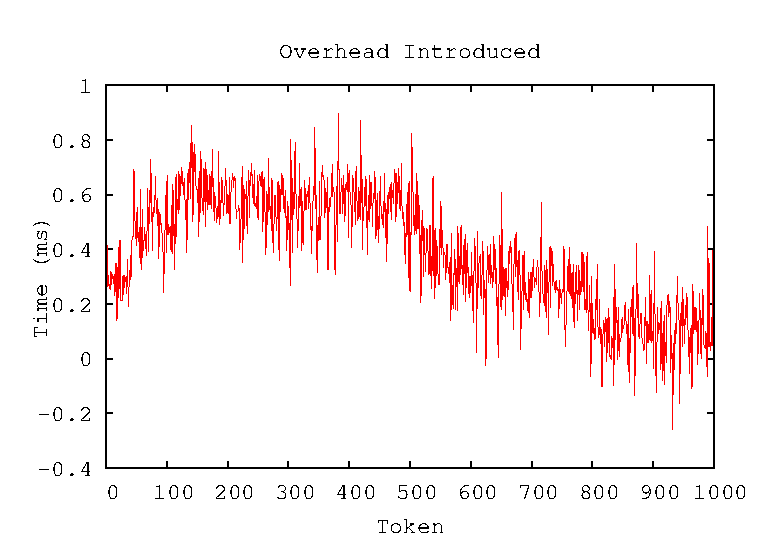
\includegraphics[width=\linewidth]{figures/overhead}
%        \caption{Overhead introduced by resilience changes.}
%        \label{fig:overhead}
%    \end{minipage}
\end{figure}

Our changes to the Open MPI Runtime Environment (ORTE) demonstrate the low
amount of overhead introduced in failure free execution as well as fast failure
detection when failures do occur.

We created a micro-benchmark to measure failure detection time on different MPI
processes. The benchmark uses an \mpifunc{MPI\_BARRIER} to roughly synchronize
the processes, stores the reference start time, then enters a ring algorithm
while injecting a failure at a predetermined location. When the failure is
detected, MPI stores the detection time to determine a relative length for the
failure detection. Figure~\ref{fig:binomial-detection} demonstrates the
detection time for failures in three different locations in the system, ranks 1
(low), 8 (middle), and 15 (high). It demonstrates a binomial OOB topology which
allows for fast, scalable failure detection due to its tree-based topology. The
experiment shows an average of 20 runs with error bars showing the standard
deviation of the runs.

%Using the same micro-benchmark for Figure~\ref{fig:overhead}, we measured the
%overhead introduced by our changes to the Open MPI source by comparing the
%timing results of our resilient code to the Open MPI trunk revision 24614. The
%only change in the benchmark is that failures were not introduced during the
%execution and only the round trip time of the tokens were used. The results show
%that the changes introduced a very small amount of overhead of about 0.5ms. The
%variations in the overhead can be explained by network jitter while the overhead
%mostly comes from small increase in the header size due to data necessary for
%the resilient code.

\subsection{\cof Results}\label{subsect:cof-results}

\begin{figure}
    \centering
%    \begin{minipage}{.48\linewidth}
    \begin{minipage}{.73\linewidth}
        \includegraphics[width=\linewidth]{figures/kraken-new-data}
        \caption{\cof QR on Kraken (Lustre)}
        \label{fig:cof-kraken}
    \end{minipage}
%    \hfill
%    \begin{minipage}{.48\linewidth}
%        \includegraphics[width=\linewidth]{figures/dancer-performance-data}
%        \caption{\cof QR on Dancer (local SSD)}
%        \label{fig:cof-dancer}
%    \end{minipage}
\end{figure}

To demonstrate the usefulness of the \cof work, Peng Du implemented a \cof
compatible version of a QR factorization. Details of the \cof-QR can be found
in~\cite{Bland:2012tw}. Figure~\ref{fig:cof-kraken} presents the performance of
the \cof-QR code on the Kraken supercomputer. This test was run on a process
grid of 24x24 with a block size of 100. The figure illustrates both the
failure-free and failure-resilient executions compared to the reference
ScaLAPACK implementation.

The result of this experiment demonstrates the feasibility of \cof as a recovery
scheme for some \abft applications. The \cof-QR code was able to achieve
performance results of at least 90\% of the reference ScaLAPACK implementation,
even in the presence of failures, with even better results in the failure-free
case. This shows that compared to a possible performance loss of 25\% or more
with traditional checkpointing, \cof can significantly improve runtime.

\subsection{\ulfm Results}\label{subsect:ulfm-results}

The \ulfm proposal is in its early stages of implementation and testing, however
there have been some comparisons between \ulfm-compatible MPI and 2.2-Standard
MPI to measure the overhead introduced by the new requirements. These tests were
performed on the Smoky system at Oak Ridge National Laboratory. Each node
contains four quad-core 2.0 GHz AMD Opteron processors with 2 GB of memory per
compute core. Nodes are connected with gigabit Ethernet and InfiniBand. Some
shared-memory benchmarks were conducted on Romulus, a $6\times8$ AMD Opteron
6180 SE with 256 GB of memory (32 GB per socket) at the University of Tennessee.
We compare the vanilla version of Open MPI (r26237) with the ULFM enabled
version. 

%Table~\ref{tab:netpipe} demonstrates the low impact on 1-byte latency and
%bandwidth using the NetPIPE benchmark (v3.7). 

Experiments using the NetPIPE benchmark have demonstrated that for all types of
interconnect, the difference between the \ulfm implementation performance and
the vanilla version of Open MPI is negligible. All of the differences are within
the standard deviation of both measurements which shows that any variation is as
likely to be caused by network noise as implementation changes.

%\begin{table*}
%    \begin{center}
%        \begin{tabular}{|l||r|r||r|r||r|}
%            \multicolumn{6}{c}{1-byte Latency (microseconds) (cache hot)} \\
%            \hline
%            \cellcolor[gray]{0.7}\textbf{Interconnect}  & \cellcolor[gray]{0.7}\textbf{Vanilla}   & \cellcolor[gray]{0.7}\textbf{Std. Dev.} &
%            \cellcolor[gray]{0.7}\textbf{\ulfm}         & \cellcolor[gray]{0.7}\textbf{Std. Dev.} & \cellcolor[gray]{0.7}\textbf{Difference} \\
%            \hline
%
%            \cellcolor[gray]{0.9}Shared Memory &  0.8008 & 0.0093 &  0.8016 & 0.0161 &  0.0008 \\
%            \cellcolor[gray]{0.9}TCP           & 10.2564 & 0.0946 & 10.2776 & 0.1065 &  0.0212 \\
%            \cellcolor[gray]{0.9}OpenIB        &  4.9637 & 0.0018 &  4.9650 & 0.0022 &  0.0013 \\
%            \hline
%            \multicolumn{6}{c}{Bandwidth (Mbps) (cache hot)} \\
%            \hline
%            \cellcolor[gray]{0.7}\textbf{Interconnect}  & \cellcolor[gray]{0.7}\textbf{Vanilla}   & \cellcolor[gray]{0.7}\textbf{Std. Dev.} &
%            \cellcolor[gray]{0.7}\textbf{\ulfm}         & \cellcolor[gray]{0.7}\textbf{Std. Dev.} & \cellcolor[gray]{0.7}\textbf{Difference} \\
%            \hline
%            \cellcolor[gray]{0.9}Shared Memory &  10,625.92 &  23.46 &  10,602.68 & 30.73 & -23.24 \\
%            \cellcolor[gray]{0.9}TCP           &   6,311.38 &  14.42 &   6,302.75 & 10.72 &  -8.63 \\
%            \cellcolor[gray]{0.9}OpenIB        &   9,688.85 &   3.29 &   9,689.13 &  3.77 &   0.28 \\
%            \hline
%        \end{tabular}
%    \end{center}
%    \caption{NetPIPE results on Smoky.\label{tab:netpipe}}
%\end{table*}

%\begin{figure}
%    \includegraphics[width=\linewidth]{figures/IMB}
%    \caption{The Intel MPI Benchmarks: relative difference between \ulfm and the
%    vanilla Open MPI on shared memory (Romulus). Standard deviation $\approx$5\%
%    on 1,000 runs.}
%    \label{fig:IMB}
%\end{figure}

%To test the impact on shared memory systems, we used the IMB benchmark suite
%(v3.2.3). Figure~\ref{fig:IMB} shows the duration difference for all the
%benchmarks remains below 5\% in either direction, the standard deviation of the
%implementation on Romulus.

\begin{figure}
    \includegraphics[width=\linewidth]{figures/bargraph.pdf}
    \caption{Comparison of the vanilla and \ulfm versions of Open MPI running
    Sequoia-AMG at different scales (Smoky).}
    \label{fig:sequoia:bargraph}
\end{figure}

To measure the impact of the prototype on a real application, we used the
Sequoia AMG benchmark\footnote{https://asc.llnl.gov/sequoia/benchmarks/\#amg}.
This MPI intensive benchmark is an Algebraic Mult-Grid (AMG) linear system
solver for unstructured mesh physics. A weak scaling study was conducted up to
512 processes following the problem \emph{Set 5}. In
Figure~\ref{fig:sequoia:bargraph}, we compare the time slicing of three main
phases (Solve, Setup, and SStruct) of the benchmark, with, side by side, the
vanilla version of the Open MPI implementation, and the \ulfm enabled one. The
application itself is not fault tolerant and does not use the features proposed
in \ulfm. The goal of this benchmark is to demonstrate that a careful
implementation of the proposed semantic does not impact the performance of the
MPI implementation, and ultimately leaves the behavior and performance of legacy
applications unchanged. The results show that the performance difference is
negligible.

Both of these results are encouraging for future work along the \ulfm path. They
provide proof that an implementation of the new constructs for \ulfm does not
need to cause an increase in overhead generated by the MPI implementation. This
should lead to greater adoption of the \ulfm proposal by multiple MPI
implementations.

%\begin{figure}
%    \includegraphics[width=\linewidth]{figures/scalability.pdf}
%    \caption{Evaluation of the Fault Injection Benchmark with full
%    recovery at different scales (Smoky).}
%    \label{fig:frssj:scalability}
%\end{figure}

\begin{comment}

To assess the overheads of recovery constructs, we developed a synthetic
benchmark that mimics the behavior of a typical fixed-size tightly-coupled
fault-tolerant application. Unlike a normal application it performs an infinite
loop, where each iteration contains a failure and the corresponding recovery
procedure. Each iteration consists of 5 phases: in the first phase
(\emph{Detection}), all processes but a designated victim enter a Barrier on the
intracommunicator. The victim dies, and the failure detection mechanism makes
all surviving processes exit the Barrier, some with an error code. In Phase 2
(\emph{Revoke}), the surviving processes that detected a process-failure related
error during the previous phase invoke the new construct
\mpifunc{MPI\_COMM\_REVOKE}. Then they proceed to Phase 3 (\emph{Shrink}) where
the intracommunicator is shrunk using \mpifunc{MPI\_COMM\_SHRINK}. The two other
phases serve to repair a full-size intracommunicator using spawn and
intercommunicator merge operations to allow the benchmark to proceed to the next
round.

In Figure~\ref{fig:frssj:scalability}, we present the timing of each phase,
averaged upon 50 iterations of the benchmark loop, for a varying number of
processes on the Smoky machine. We focus on the three points related to \ulfm:
failure detection, revoke and shrink. The failure detection is mildly impacted
by the scale. In the prototype implementation, the detection happens at two
levels, either in the runtime system or in the MPI library (when it occurs on an
active link).  Between the two detectors, all ranks get notified within 30ms of
the failure (this compares to the 1s timeout at the link level). Although the
revoke call will inject a linear number of messages (at each rank) in the
network to implement the level of reliability required for this operation, the
duration of this call itself is under 50$\mu$s and is not visible in the figure.
The network is disturbed for a longer period, due to the processing of the
messages, but this disturbance will appear in the network only after a failure
occurred.  The last call shown in the figure is the shrink operation. Although
its duration increases linearly with the number of processes (the figure has a
logarithmic scale on the x-axis), this cost must only be paid after a failure,
in order to continue using collective operations. In its current implementation,
shrink requires an agreement, the allocation of a new communicator identifier,
and the creation of the communicator (with \mpifunc{MPI\_COMM\_SPLIT}). Most of
the time spent in the shrink operation is not in the agreement (which scales
logarithmically), but in the underlying implementation of the communicator
creation. 

\end{comment}

\section{Conclusion}
\label{sect:conclusion}

Many responsible voices agree that sharp increases in the volatility of future,
extreme scale computing platforms are likely to imperil our ability to use them
for advanced applications that deliver meaningful scientific results and
maximize research productivity. Since MPI is currently, and will likely continue
to be -- in the medium-term -- both the de-facto programming model for
distributed applications and the default execution model for large scale
platforms running at the bleeding edge, it is the place in the software
infrastructure where semantic and run-time support for application faults needs
to be provided.

The \ulfm proposal is a careful but important step forward toward accomplishing
this goal delivering support for a number of new and innovative resilience
techniques through simple, familiar API calls, but it is backward compatible
with previous versions of the MPI standard, so that non fault-tolerant
applications (legacy or otherwise) are supported without any changes to the
code. Perhaps most significantly, applications can use \ulfm-enabled MPI without
experiencing any degradation in their performance, as we demonstrate in this
paper. Some of these applications along with other portable libraries are
currently being refactored to take advantage of \ulfm semantics.

The author would like to acknowledge his co-authors in the full
paper~\cite{Bland:2012tp}: Aurelien Bouteiller, Thomas Herault, Joshua Hursey,
George Bosilca, and Jack J. Dongarra.

\section{Related Publications}\label{sect:publications}

\begin{itemize}

\item An Evaluation of User-Level Failure Mitigation Support in MPI, EuroMPI
    2012~\cite{Bland:2012tp}

\item A Checkpoint-on-Failure Protocol for Algorithm-Based Recovery in Standard
    MPI, Distinguished Paper Award, Euro-Par 2012~\cite{Bland:2012tw}

\item Enabling Application Resilience With and Without the MPI Standard, CCGrid
    2012~\cite{Bland:2012gy}

\end{itemize}


\clearpage

\newcommand{\BIBdecl}{\setlength{\itemsep}{0.03\baselineskip}} 
\bibliographystyle{IEEEtranS}
\bibliography{phd-proposal}

\end{document}

